\documentclass{exam}
\usepackage{babel}
\usepackage[utf8]{inputenc}
\usepackage{amsmath, amsthm, amssymb}
\usepackage{ragged2e}
\usepackage{lmodern}
\usepackage{tcolorbox}
\usepackage{hyperref}
\usepackage{verbatim}
\usepackage{tikz}
\usepackage{enumitem}

\pagestyle{empty}
\renewcommand{\theenumi}{\alph{enumi}}
\renewenvironment{proof}{{\noindent\itshape\ignorespaces}}{{\hfill$\qed$\\}}

\DeclareMathOperator*{\argmin}{arg\,min}

\begin{document}

\begin{center}
    \textbf{\Large Exercises 5.10 }
\end{center}

\section*{Exercise 5.10.1}
Recall that $\neg x$ is the negative of the Boolean variable $x$. 
\begin{enumerate}
    \item Show that a single perceptron can learn the Boolean function $y = x_{1}\land \neg x_{2}$, with some $x_{1} \text{ , } x_{2} \in \{0,1\}$.
    \item The same question as in part $a$ for the Boolean function $y = x_{1}\lor \neg x_{2}$, with some $x_{1} \text{ , } x_{2} \in \{0,1\}$.
    \item Show that a perceptron with one Boolean input, $x$, can learn the negation function $y = \neg x$. What about the linear neuron?
    \item Show that a perceptron with three Boolean inputs, $x_{1} \text{ , } x_{2} \text{ , } x_3$, can learn the negation function $y = \neg x$. What about $x_1 \lor x_2 \lor x_3$?
\end{enumerate}

\section*{Exercise 5.10.2}
Show that two finite linearly separable sets $A$ and $B$ can be separated by a perceptron with rational weights. 

\section*{Exercise 5.10.3}
Assume the inputs to a linear neuron are independent and normaly distributed, $X_{i} \sim \mathcal{N}(0, \sigma^{2}_{i}), \ i = 1, \ldots , n$. Find the 
optimal weights, $w^{\star}$
\begin{enumerate}
   \item A one dimensional random variable with zero mean, $Z$ is learned by a linear neuron with input $X$. Assume the input, $X$, and the target $Z$
   are independent. Write the cost function and find the optimal parameters, $w^{\star}$. Provide an interpretation of the result.
   \item Use Newton's method to obtain the optimal parametersof a linear neuron.
\end{enumerate}  

\section*{Exercise 5.10.4}
Explain the equivalence between the linear regression algorithm an the learning of a linear neuron.

\section*{Exercise 5.10.5}
Consider a neuron with a continuum input, whose output is $y = H(\displaystyle \int_{0}^{1}x d \mu(x))$. Find the output in the case when the measure 
is $\mu = \delta_{x_0}$. \newpage

\section*{Exercise 5.10.6}
Consider $n$ points $P_1,\ldots P_n$, included in a half-circle, and denote by $\bold{x}_1, \ldots, \bold{x}_n$ their coordinate vectors.
\begin{figure}[h]
    \centering
    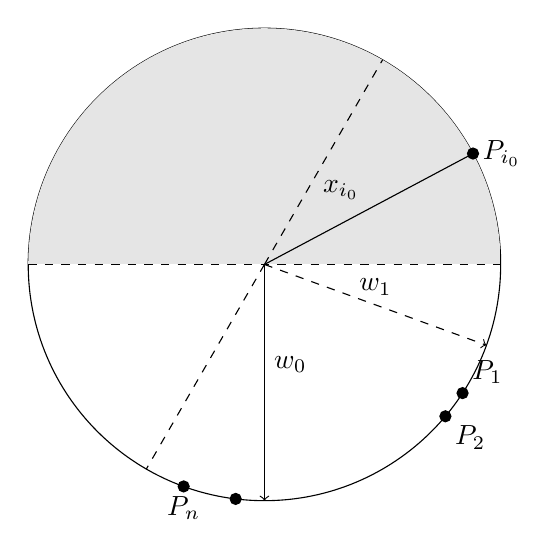
\begin{tikzpicture}
        % Draw the circle
        \draw (0,0) circle (3cm);
        
        % Shade half of the circle
        \begin{scope}
            \clip (0,0) circle (3cm);
            \fill[gray!20] (-3,0) rectangle (3,3);
        \end{scope}
        
        % Draw the existing diameter
        \draw[dashed] (-3,0) -- (3,0);
        
        % Draw the new diameter at 60 degrees
        \draw[dashed] (0,0) -- (60:3cm);
        \draw[dashed] (0,0) -- (240:3cm); % This is the continuation of the diameter on the other side
        
        % Place points on the circle
        \filldraw (0,0) -- (28:3cm) circle (2pt) node[midway, above left]{$x_{i_0}$} node[above, right]{$P_{i_0}$};
        \filldraw (-33:3cm) circle (2pt) node[above right] {$P_1$};
        \filldraw (-40:3cm) circle (2pt) node[below right] {$P_2$};
        \filldraw (-97:3cm) circle (2pt) node[below] {};
        \filldraw (-110:3cm) circle (2pt) node[below] {$P_n$};
        % Draw and label the radius vectors forming an acute angle in the unshaded half-circle
        \draw[dashed, ->] (0,0) -- (-20:3cm) node[midway, above] {$w_1$};
        \filldraw[->] (0,0) -- (-90:3cm) node[midway, above right] {$w_0$};
    \end{tikzpicture}
    
    \caption{Perceptron algorithm}
\end{figure}   

A perceptron can learn the aforementioned half-circle by the following algorithm:\\

\begin{enumerate}[label*=\arabic*.]
    \item Start from an arbitaryhalf-circle determined by its diameter and a unit normal vector $w_0$. Then select an incorreclty classified point, $P_{i_0}$, i.e.
    , a point for which $\left< w_0, \bold{x}_{i_0}\right> < 0$. See Fig 1. 
    \item Rotate the diameter that the new normal is $w_1 = w_0 + \bold{x}_{i_0}$. Show that the point is now correclty classified.
    \item Repeating the previoustwo steps, we constructed inductively the sequence of vectors $(w_m)_{m}$. Such that $w_{m+1} = w_m + \bold{x}_{i_m}$, where $P_{i_m}$ is 
    a point misclassified at step $m$. Show that the process ends in a finite number of steps, i.e. , there is a $N > 1$ such that $\left< w_0, \bold{x}_{j}\right> > 0, \  \forall \ 1 \leq j \leq n.$ 
    Find an estimate of the number N.
\end{enumerate}

\section*{Exercise 5.10.7}
Modify the perceptron learning algorithm given by Exercise $5.10.6$ for the case when the points $P_1, \ldots P_n$ are included in a half-plane.

\section*{Exercise 5.10.8}
Let $\boldsymbol{1}_{A}(x)$ denote the characteristic function of the set $A$, namely, $\boldsymbol{1}_{A}(x) = 1$ if $x \in A$ and $\boldsymbol{1}_{A}(x) = 0$ if $x \notin A$
\begin{enumerate}
    \item Show that the function
    $\phi(x_1,x_2) = \boldsymbol{1}_{x_2 > x_1 + 0.5}(x_1,x_2) + \boldsymbol{1}_{x_2 > x_1 - 0.5}(x_1,x_2)$ \\
    implements $XOR$.
    \item Show that the $XOR$ function can be implement by a linear combination of the two perceptrons.
\end{enumerate}

\section*{Exercise 5.10.9}
Show that if all input vectors $x_k$ have the same length, then the $\alpha-LMS$ algorithm minimizes the mean square error and in this case the updating 
rule $(5.6.6)$ becomes the gradient descent rule.
\section*{Exercise 5.10.10}
Find the weights of a Madaline with two Adaline units which implements the $XNOR$ function.
\begin{center}    
    \section*{SOLUTIONS}
\end{center}

\end{document}